\subsubsection{General Solution}

Our differential equation for the system:

\begin{equation}
    v(t) + \tau_m \cdot \dot{v}(t) = I(t)
\end{equation}

The Fourier transform of our differential equation:

\begin{equation}
    \mathcal{F}[v(t)](\omega) = V(\omega), \quad \mathcal{F}[\dot{v}(t)](\omega) = i\omega \cdot V(\omega)
\end{equation}

\begin{equation}
    \mathcal{F}[I(t)] = I(\omega)
\end{equation}

\begin{equation}
    \mathcal{F}[v(t) + \tau_m \dot{v}(t)](\omega) = \mathcal{F}[I(t)](\omega)
\end{equation}

\begin{equation}
    V(\omega) + \tau_m \cdot i \omega \cdot V(\omega) = I(\omega)
\end{equation}

\begin{equation}
(1 + i\omega \tau_m) V(\omega) = I(\omega)
\end{equation}

The Transfer function of the system:
\begin{equation}
H(\omega) = \frac{V(\omega)}{I(\omega)} = \frac{1/\tau_m}{1/\tau_m + i\omega}
\end{equation}

We can separate the factors of this complex definition to:
\begin{equation}
H(\omega) = |H(\omega)| \cdot e^{i \cdot \arg(H(\omega))}
\end{equation}
\begin{equation}
|H(\omega = 0)| = 1, \quad \lim_{\omega \to \infty} |H(\omega)| = 0, \quad \lim_{\omega \to -\infty} |H(\omega)| = 0
\end{equation}

As we can see, the transfer function behaves as a low pass filter!
In addition, we can look at the argument of the complex number that will translate into a time shift in the time domain:
\begin{equation}
\phi(\omega) = \arg(H(\omega)) = \arctan(-\omega/\tau_m) = -\arctan(\tau_m \omega)
\end{equation}
\begin{equation}
\phi(\omega = 0) = 0, \quad \lim_{\omega \to \infty} \phi(\omega) = -\frac{\pi}{2}, \quad \lim_{\omega \to -\infty} \phi(\omega) = \frac{\pi}{2}
\end{equation}

To demonstrate the meaning of the transfer function and analysis we developed, we will look at:

\begin{equation}
    I(t) = I_0 \cos(\omega_0 t)
\end{equation}

\begin{equation}
    I(t) = \frac{1}{2} \cdot I_0 \cdot \left(e^{i\omega_0 t} + e^{-i\omega_0 t}\right)
\end{equation}

\begin{equation}
    \mathcal{F}[I(t)](\omega) = I(\omega) = \frac{1}{2} \cdot I_0 \cdot \left(\delta(\omega - \omega_0) + \delta(\omega + \omega_0)\right)
\end{equation}

\begin{equation}
    V(\omega) = H(\omega) \cdot I(\omega) = \frac{1}{2}  \cdot I_0 \cdot |H(\omega_0)| \left(e^{i\phi(\omega_0)} \delta(\omega - \omega_0) + e^{-i\phi(\omega_0)} \delta(\omega + \omega_0)\right)
\end{equation}

\begin{equation}
\begin{aligned}
    v(t) = \mathcal{F}^{-1}[H(\omega) \cdot I(\omega)] = I_0 |H(\omega_0)| \cdot \left(e^{i(\omega_0 t + \phi(\omega_0))} + e^{-i(\omega_0 t + \phi(\omega_0))}\right) = \\ = I_0 |H(\omega_0)| \cos(\omega_0 t + \phi(\omega_0))
\end{aligned}
\end{equation} \\

Input with high frequency will result in an output with smaller amplitude:

\begin{figure}[H]
    \centering
    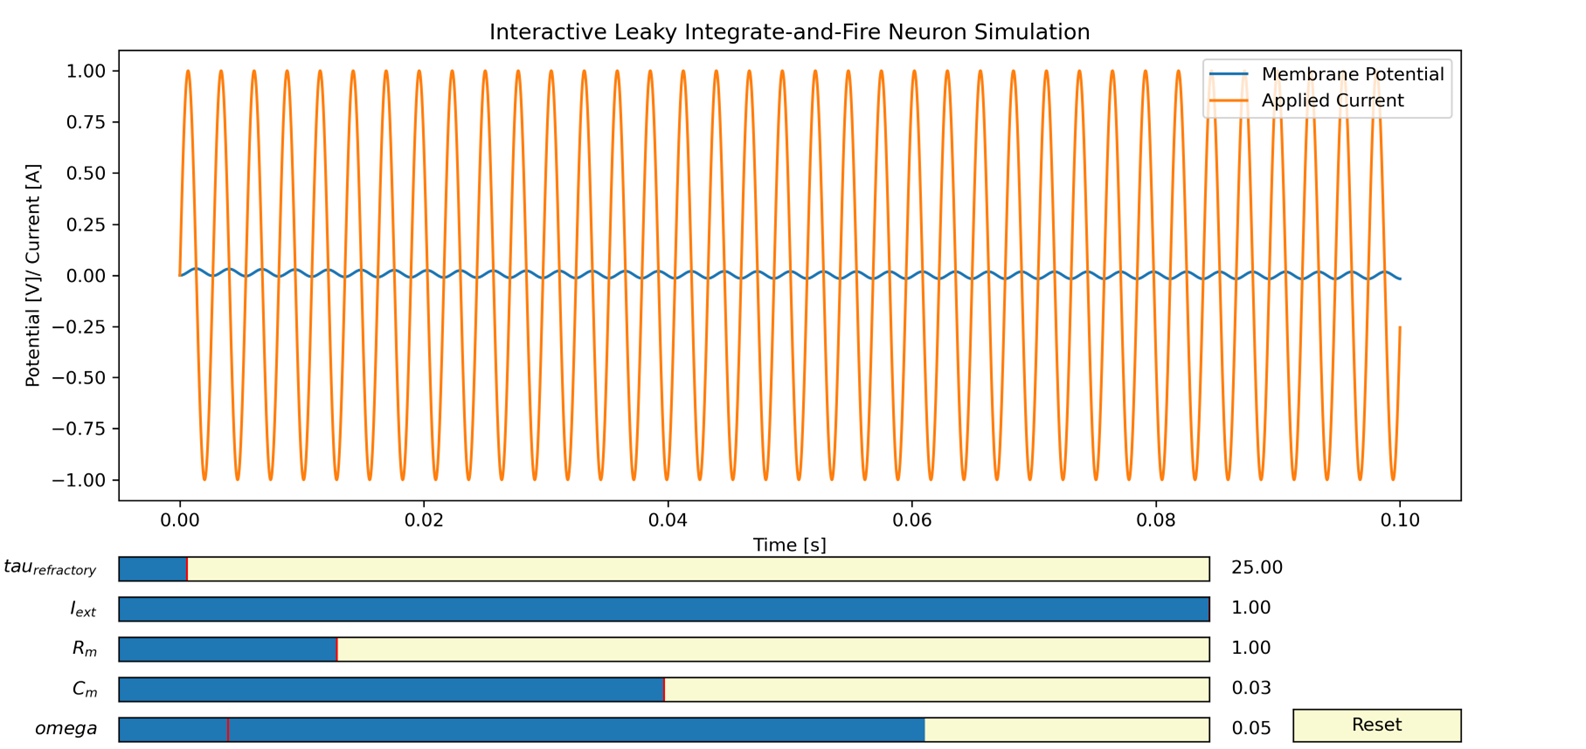
\includegraphics[width=0.8\textwidth]{scientific-background/computational-models/LIF/graphs/LIF-high-freq-sin-response.png}
    \caption{LIF membrane voltage response to high frequency sinusoidal function with high amplitude}
    \label{fig:LIF-high-freq-sin}
\end{figure}

The output of a periodic function is also periodic with the same frequency:

\begin{figure}[H]
    \centering
    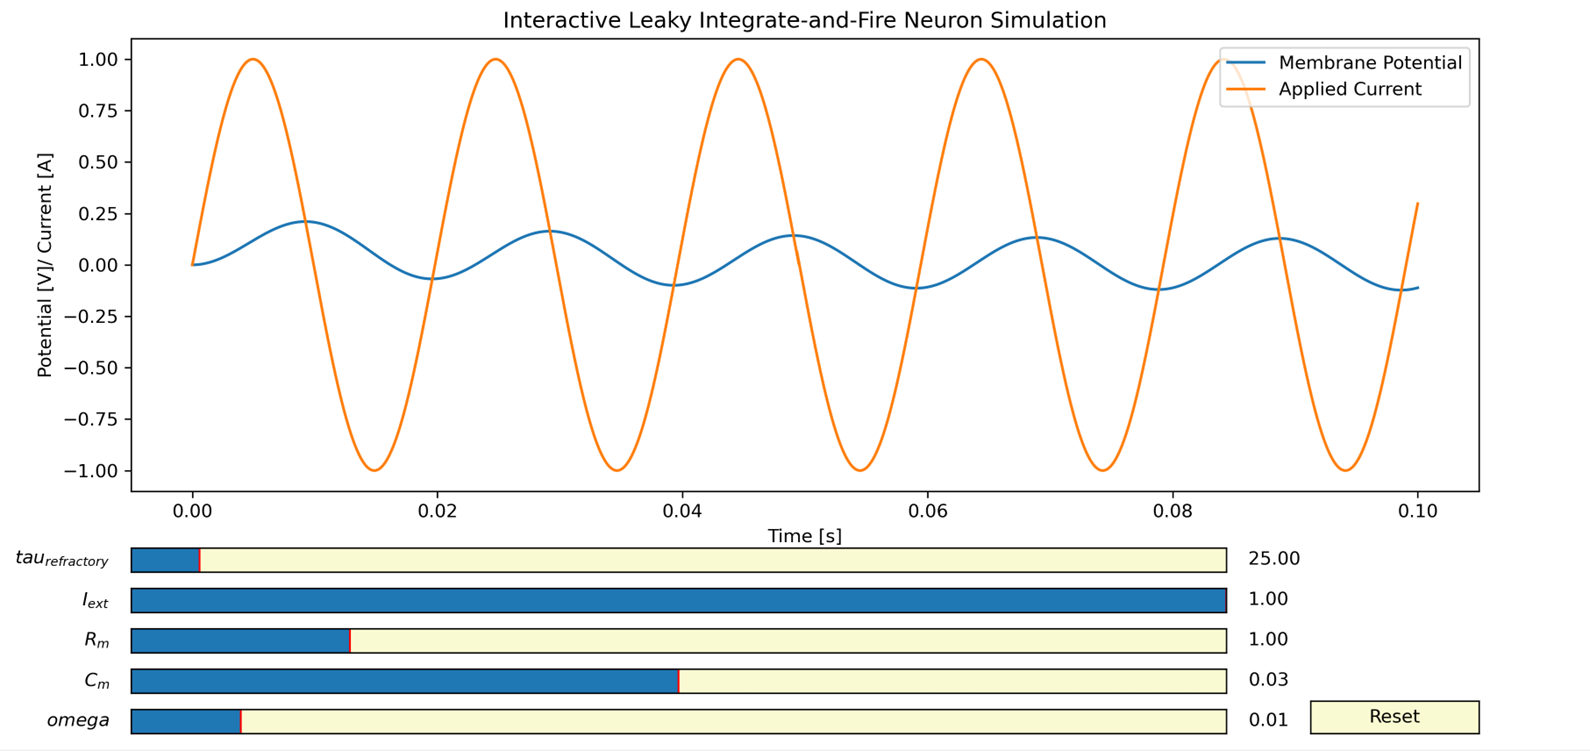
\includegraphics[width=0.8\textwidth]{scientific-background/computational-models/LIF/graphs/LIF-med-freq-sin-response.png}
    \caption{LIF membrane voltage response sinusoidal function with high amplitude}
    \label{fig:LIF-med-freq-sin}
\end{figure}

Smaller frequency input will give an output with bigger amplitude (close to the input’s amplitude) and smaller time shift:

\begin{figure}[H]
    \centering
    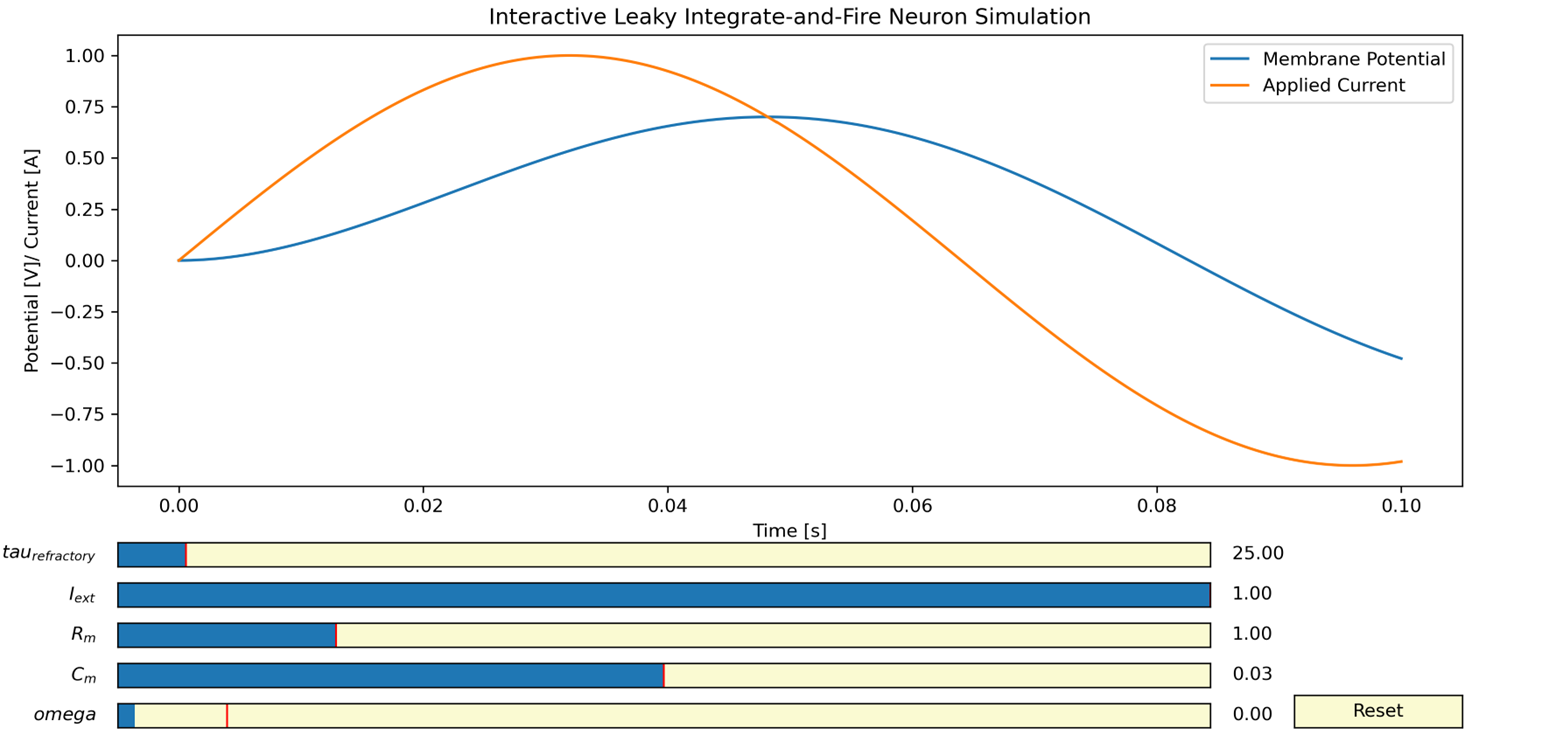
\includegraphics[width=0.8\textwidth]{scientific-background/computational-models/LIF/graphs/LIF-low-freq-sin-response.png}
    \caption{LIF membrane voltage response to low frequency sinusoidal function with high amplitude}
    \label{fig:LIF-low-freq-sin}
\end{figure}